\documentclass{standalone}
\usepackage{tikz}
\usepackage{amsmath, amssymb}
\usepackage{xcolor}

% Load the MSE color scheme
% MSE Colors - Matching the MkDocs website
% This file contains color definitions matching the MkDocs site: MSE1_DK_25

%% Light Mode Colors
\definecolor{mseViaBlue}{RGB}{108, 162, 198}    % #6CA2C6 - VIA blue for links/accents
\definecolor{mseOrange}{RGB}{255, 140, 0}       % #FF8C00 - Orange accent
\definecolor{mseDarkText}{RGB}{54, 54, 54}      % #363636 - Default text color
\definecolor{mseBackground}{RGB}{255, 255, 255} % #FFFFFF - Background

%% Dark Mode Colors
\definecolor{mseDarkBg}{RGB}{13, 16, 23}        % #0d1017 - Dark background
\definecolor{mseDarkBlue}{RGB}{18, 49, 97}      % #123161 - Header/active elements
\definecolor{mseGlowBlue}{RGB}{42, 157, 244}    % #2A9DF4 - Glow/secondary blue
\definecolor{mseLightBlue}{RGB}{60, 172, 248}   % #3CACF8 - Light blue accent
\definecolor{mseDarkText}{RGB}{192, 212, 240}   % #C0D4F0 - Dark mode foreground text

%% Admonition Colors
\definecolor{mseQuestionBorder}{RGB}{45, 180, 153}   % #2DB499 - Question green
\definecolor{mseQuestionBg}{RGB}{204, 241, 234}      % #CCF1EA - Question background
\definecolor{mseAnswerBorder}{RGB}{229, 171, 72}     % #E5AB48 - Answer orange
\definecolor{mseAnswerBg}{RGB}{255, 239, 211}        % #FFEFD3 - Answer background

%% Set Number Theory Colors (for Venn diagrams, etc)
\definecolor{mseNaturals}{RGB}{255, 150, 50}       % BurntOrange - Natural Numbers
\definecolor{mseIntegers}{RGB}{255, 120, 70}       % Bittersweet - Integers
\definecolor{mseRationals}{RGB}{210, 160, 110}     % RawSienna - Rational Numbers
\definecolor{mseIrrationals}{RGB}{210, 150, 70}    % Custom orange - Irrational Numbers
\definecolor{mseReals}{RGB}{158, 196, 233}         % Light blue - Real Numbers (changed from duplicate RawSienna)
\definecolor{mseImaginary}{RGB}{150, 190, 70}      % YellowGreen - Imaginary Numbers
\definecolor{mseComplex}{RGB}{100, 180, 100}       % OliveGreen - Complex Numbers


\begin{document}

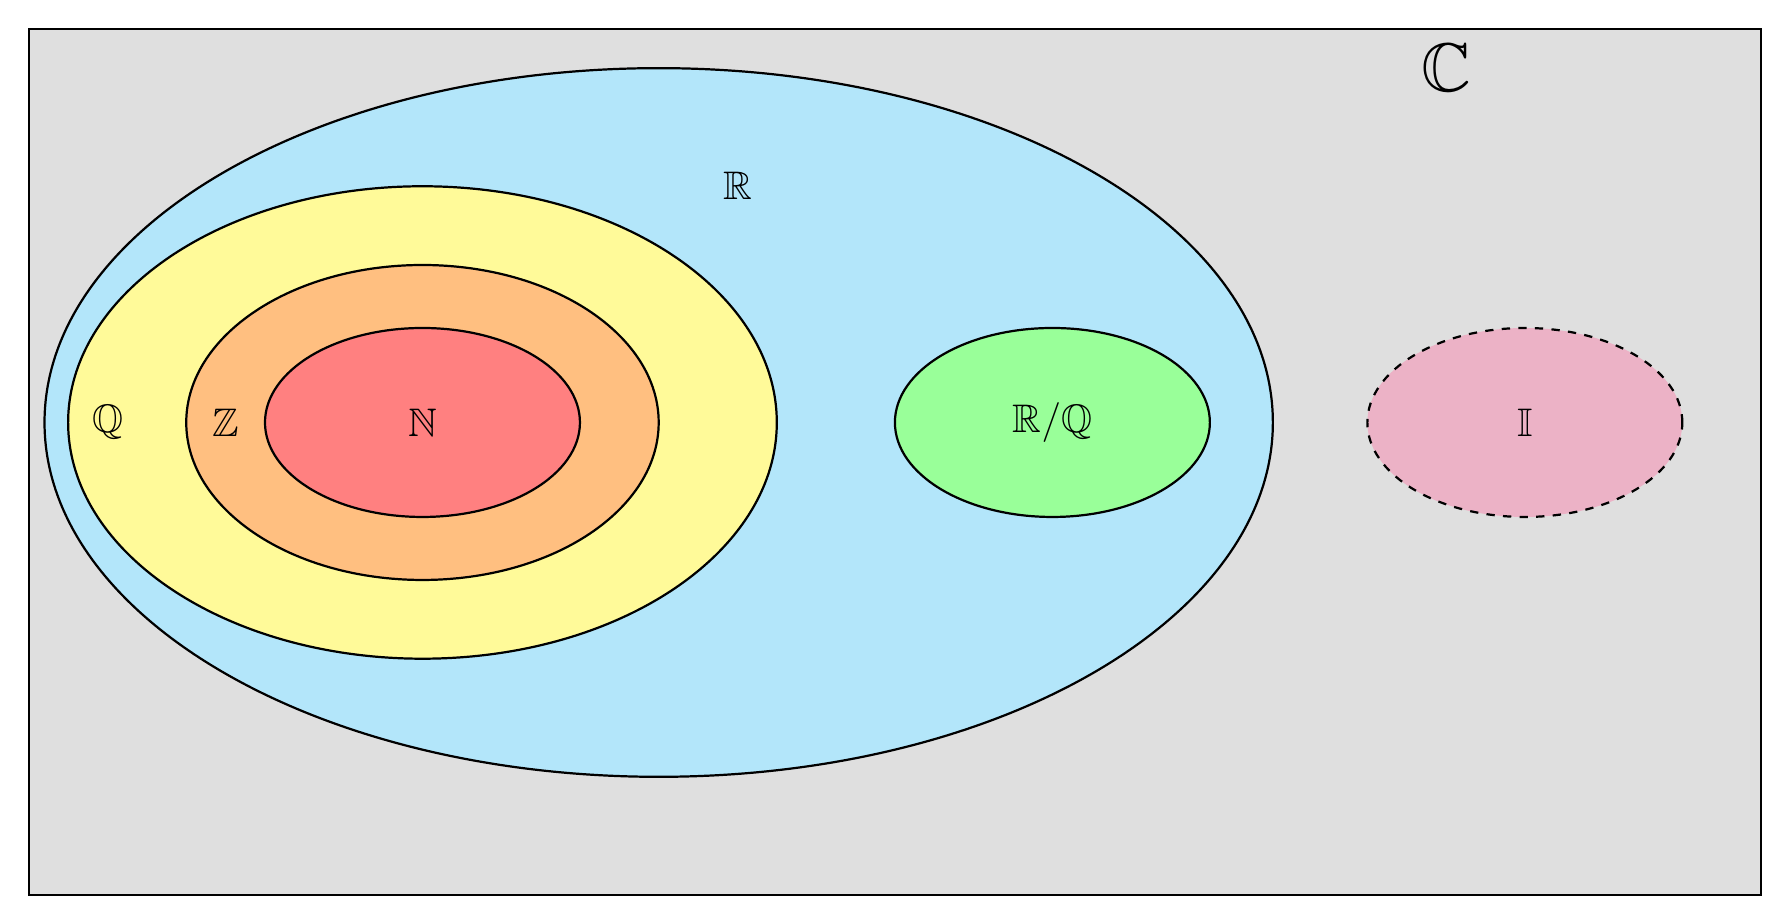
\begin{tikzpicture}

    % Complex Numbers (outer square)
    \draw[thick, fill=lightgray!50] (-12, -6) rectangle (10, 5);
    \node at (6, 4.5) {\Huge $\mathbb{C}$};
    
    % Real Numbers (largest set)
    \draw[thick, fill=cyan!30] (-4,0) ellipse (7.8cm and 4.5cm);
    \node at (-3, 3) {\Large $\mathbb{R}$};
    
    % Rational Numbers
    \draw[thick, fill=yellow!40] (-7,0) ellipse (4.5cm and 3cm);
    \node at (-11, 0) {\Large$\mathbb{Q}$};
    
    % Integers
    \draw[thick, fill=orange!50] (-7,0) ellipse (3cm and 2cm);
    \node at (-9.5, 0) {\Large$\mathbb{Z}$};
    
    % Natural Numbers
    \draw[thick, fill=red!50] (-7,0) ellipse (2cm and 1.2cm);
    \node at (-7, 0) {\Large$\mathbb{N}$};
    
    % Irrational Numbers
    \draw[thick, fill=green!40] (1,0) ellipse (2cm and 1.2cm);
    \node at (1, 0) {\Large$\mathbb{R} /\mathbb{Q} $};
    
    % Imaginary Numbers
    \draw[thick, dashed, fill=purple!30] (7,0) ellipse (2cm and 1.2cm);
    \node at (7, 0) {\Large $\mathbb{I}$};

\end{tikzpicture}

\end{document}
